%qqqqqqqqqqqqqqqqqqqqqqqqqqqqqqqqqqqqqqqqqqqqqqqqqqqqqqqqqqqqqqqqqqqqqqqqq
%Quote
\begin{savequote}[50mm]
‘‘El cosmos es todo lo que es, todo lo que fue y todo lo que será. Nuestras 
más ligeras contemplaciones del cosmos nos hacen estremecer: Sentimos como 
un cosquilleo nos llena los nervios, una voz muda, una ligera sensación como
de un recuerdo lejano o como si cayéramos desde gran altura. Sabemos que nos
aproximamos al más grande de los misterios.’’
\qauthor{Carl Sagan}
\end{savequote}
%qqqqqqqqqqqqqqqqqqqqqqqqqqqqqqqqqqqqqqqqqqqqqqqqqqqqqqqqqqqqqqqqqqqqqqqqq




%#########################################################################
\chapter{Marco Teórico}
\label{cha:Theoretical Framework}


Este capítulo se concentra en abarcar de forma autocontenida y resumida 
todo el marco teórico necesario para el estudio del universo a gran escala,
pasando por los modelos simples de universo dados por las soluciones de 
Friedmann, la teoría de perturbaciones para la generación de estructuras
complejas como galaxias y cúmulos galácticos, hasta la cuantificación del 
red cósmica.
%#########################################################################




%*************************************************************************
%Isotropic and homogeneous universe
\section{Universo Isotrópico y Homogéneo}
\label{sec:IsotropicAndHomogeneousUniverse}


Los dos grandes pilares de la comoslogía moderna son el principio cosmológico
y la teoría de la relatividad general. El primero es un principio que asume 
que el universo es homogéneo e isotrópico a grandes escalas, mientras que la 
segunda da el soporte teórico necesario para un entendimiento adecuado de la 
relación entre materia y la estructura del espacio-tiempo.


Como han indicado observaciones de estructura a gran escala y de radiación
cósmica de fondo nuestro universo parece ser isotrópico y homogéneo a muy
grandes escalas, lo que está acorde con el principio cosmológico. Más aún, 
esta hecho simplifica bastante la compleja formulación tensorial de la 
relatividad general para llegar finalmente a las ecuaciones de Friedmann.


	%---------------------------------------------------------------------
	%Curved space metric
	\subsection{Métrica de Espacios Curvados}
	\label{subsec:MetricOFCurvedSpaces}
	%---------------------------------------------------------------------
	

En la construcción de un modelo isotrópico y homogéneo del universo es
necesario establecer una métrica adecuada que lo describa, como un ejemplo
ilustrativo que puede ser generalizado se considera una superficie esférica, 
que claramente satisface los criterios de homogeneidad e isotropía.


%.........................................................................
%2D sphere
\begin{figure}[htbp]
	\centering
	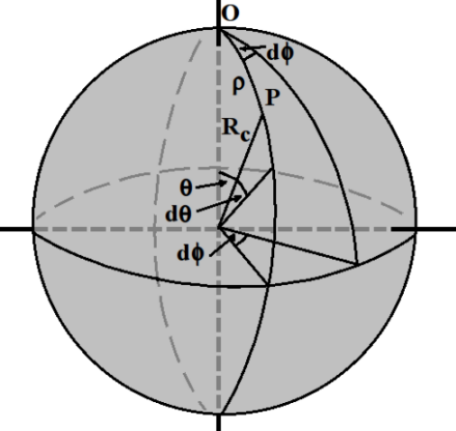
\includegraphics[width=0.5\textwidth]
	{./figures/2_theoretical_framework/2D_Sphere.png}
	
	\caption{\small{Métrica de una superficie esférica.}}
	
	\label{fig:2sphere}
\end{figure}
%.........................................................................



Un elemento de línea sobre la superficie de la figura \ref{fig:2sphere} 
puede ser descrito como


%.........................................................................
%Line element on the sphere
\[ dl^2 = d\rho^2 + R_c^2 \sin^2 \pr{ \frac{\rho}{R_c}}d\phi^2 \]
%.........................................................................


donde se ha introducido una nueva coordenada de longitud sobre la superficie
definida como $\rho = \theta R_c$ y $R_c$ radio de curvatura de la esfera. 
Otra forma muy conveniente de reescribir esta expresión y que permite una
generalización muy útil se logra introduciendo el parámetro de curvatura $k$ 
y la coordenada $r = \sin (\rho/a)$, obteniendo


%.........................................................................
%Line element on the sphere with time-dependent curvature
\[ dl^2 = a^2(t) \cor { \frac{dr^2}{1-kr^2} + r^2 d\phi^2 } \]
%.........................................................................


con $k = -1$ y se asume un radio de curvatura dependiente del tiempo 
$R_c = a(t)$.
La métrica para el caso de 3 dimensiones se obtiene reemplazando el 
diferencial del ángulo $d\phi^2$ por uno de ángulo sólido $d\Omega^2 = 
d\theta^2 + \sin^2\theta d\phi^2$

 
%.........................................................................
%Line element on the 3-sphere
\eq{eq:LineElement3D}
{ dl^2 = a^2(t) \cor { \frac{dr^2}{1-kr^2} + r^2 (d\theta^2 + 
\sin^2\theta d\phi^2)} }
%.........................................................................


Finalmente incluyendo el tiempo, el intervalo espacio-temporal para la 
métrica de espacios curvos isotrópicos y homogéneos queda


%.........................................................................
%Interval element on the 3-sphere
\eq{eq:IntervalCurvedSpaces}
{ ds^2 = c^2 dt^2 - a^2(t) \cor { \frac{dr^2}{1-kr^2} + r^2 (d\theta^2 + 
\sin^2\theta d\phi^2)} }
%.........................................................................


La generalización directa de esta expresión consiste en variar los valores
del parámetro de curvatura $k$ para llegar a la métrica de espacios planos 
($k = 0$), esféricos cerrados ($k = -1$) o abiertos ($k = 1$), tal como
es mostrado en \cite{longair2008} o \cite{padmanabhan1995}.

\
%.........................................................................
%Curved Spaces
\begin{figure}[htbp]
	\centering
	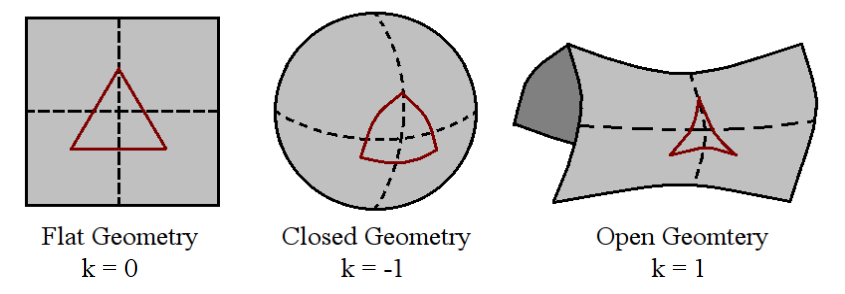
\includegraphics[width=0.9\textwidth]
	{./figures/2_theoretical_framework/Curved_Spaces.png}

	\caption{\small{Diferentes espacios curvos según el parámetro de curvatura.}}
	
	\label{fig:CurvedSpaces}
\end{figure}
%.........................................................................
\

Una manera alternativa de reescribir la métrica es introduciendo dos cambios 
de coordenadas definidos por 


%.........................................................................
%Xi variable
\[ \chi = \int \frac{ dr'}{\sqrt{1 - k r'^2}}\]
%.........................................................................


%.........................................................................
%Proper time
\[ \tau = \int \frac{ c dt'}{a(t')}\]
%.........................................................................


los cuales se interpretan respectivamente como una coordenada de longitud 
sobre la hipersuperficie que define el espacio ($\chi$) y como el tiempo 
propio medido localmente ($\tau$). Se obtiene la siguiente expresiones para 
la métrica


%.........................................................................
%Interval element generalized
\eq{eq:IntervalCurvedSpacesAltern1}
{ ds^2 = c^2 dt^2 - a^2(t) \cor { d\xi^2 +  f^2_k(\xi)(d\theta^2 + 
\sin^2\theta d\phi^2)} }
%.........................................................................


%.........................................................................
%Interval element generalized
\eq{eq:IntervalCurvedSpacesAltern2}
{ ds^2 = \bar a^2 (\tau)\cor{ d\tau^2 - d\xi^2 -  f^2_k(\xi)(d\theta^2 + 
\sin^2\theta d\phi^2)} }
%.........................................................................


donde la función $f_k(\chi)$ es definida de acuerdo al valor del parámetro 
de curvatura


%.........................................................................
%Curvature Function
\eq{eq:CurvatureFunction}
{ f_k(\chi) = \left\{  \matrix{	
\sin \chi	&	k = 1		\cr 
\chi 		& 	k = 0 		\cr	
\sinh \chi 	& 	k = -1 		\cr } \right.  }
%.........................................................................


A pesar de que las expresiones derivadas para la métrica 
\ref{eq:IntervalCurvedSpaces} \ref{eq:IntervalCurvedSpacesAltern1} y
\ref{eq:IntervalCurvedSpacesAltern2} son equivalentes, el uso de una u otra
depende de la conveniencia del problema. En especial la forma 
\ref{eq:IntervalCurvedSpacesAltern1} suele ser más usada y se define como 
métrica de Friedmann.


Puede ser mostrado que en variedades Riemannianas 
\footnote{Una variedad Riemanniana es un espacio donde puede ser definido el 
concepto de métrica.} 
el intervalo espacio-temporal se expresa en términos de la tensor métrico
como \cite{weinberg1972}


%.........................................................................
%Metric-Interval relation
\[ ds^2 = g_{\mu \nu}dx^\mu dx_\nu \]
%.........................................................................


donde se ha introducido el cuadrivector $x^\mu = (ct, r, \theta, \phi)$.


Debido a la asunción de isotropía y homogeneidad el tensor métrico debe ser
diagonal, además comparando con la expresión \ref{eq:IntervalCurvedSpaces}
se llega a la siguiente forma explícita


%.........................................................................
%MetricTensor
\eq{eq:MetricTensor}
{g_{\mu \nu} = \pr{ \matrix{ 
1		&				0			&		0			&				0				\cr
0		&	-a^2(t)(1 - kr^2)^{-1}	&	 	0			&				0				\cr
0		&				0			&	-a^2(t)r^2		&				0				\cr
0		&				0			&		0			&	-a^2(t)r^2 \sin^2 \theta } }}
%.........................................................................


A partir de esta métrica y las ecuaciones de campo de Einstein es posible 
construir sencillos modelos de universo, tal como se muestra a en la 
subsección \ref{subsec:GeneralRelativityAndFriedmannEquations}.


			%-------------------------------------------------------------
			%Medidas de distancias
			\subsubsection*{Medición de distancias}
			%-------------------------------------------------------------
			
Una vez definida la métrica de espacios curvos es útil introducir algunos
conceptos de distancia que son usados de forma recurrente \cite{longair2008}. 
Por simplicidad se asumirá una métrica plana ($k = 0$).


%Comovil Radial Distance..................................................
\textit{\textbf{Distancia radial comóvil:}} por definición, una señal 
lumínica tiene asociado un valor nulo del intervalo $ds^2 = 0$, usando la 
métrica \ref{eq:IntervalCurvedSpaces} se llega a


%.........................................................................
%Comovil Distance
\eq{eq:ComovilDistance}
{ r = \int_t^{t_0} \frac{ cdt'}{a(t')} = \int_a ^1 \frac{ c da}{a \dot a} }
%.........................................................................


donde la forma de $a(t)$ depende de la cosmología específica que se use
(ver subsección \ref{subsec:SimpleSolutionsOfTheUniverse}) y $t_0$ es el 
tiempo de referencia, el cual se toma como la edad actual del universo. 


Debido a la asunción de expansión de la métrica, la distancia entre dos 
objetos depende del tiempo en que es medida, y más aún, esta distancia no 
puede ser determinada a partir de un haz de luz debido a la finitud de su
velocidad \footnote{$c=299\ 792\ 458$ m/s}. Por esta razón se debe 
realizar una proyección del cono de luz trazado por el haz en la época 
actual, tal como se hace en la expresión \ref{eq:ComovilDistance}. Esto 
último permite interpretar $r$ como la distancia a un objeto en el tiempo
actual, y es diferente a la distancia aparente que corresponde al 
tiempo en que el objeto emitió la luz que se observa.


%Proper Radial Distance..................................................
\textit{\textbf{Distancia radial propia:}} en virtud de la definición de
factor de escala, para obtener la distancia a un objeto en cualquier 
tiempo basta multiplicar su distancia comóvil por el factor de escala en 
ese mismo tiempo, esto es


%.........................................................................
%Proper Distance
\eq{eq:ComovilDistance}
{ r_{\submath{prop}} = a(t)\int_t^{t_0} \frac{ cdt'}{a(t')} = 
a\int_a ^1 \frac{ c da}{a \dot a} }
%.........................................................................	


%Particle Horizon........................................................
\textit{\textbf{Horizonte de partículas:}} considerando un haz de luz que
viaja en el vacío desde el inicio del universo en $t=0$, la máxima 
distancia propia que puede haber recorrido en un tiempo $t$ se denomina 
horizonte de partículas y determina la región que puede estar conectada 
causalmente en el universo en esa época.


%.........................................................................
%Particle Horizon distance
\eq{eq:HorizonDistance}
{ r_{\submath{H}} = a(t)\int_0^{t} \frac{ cdt'}{a(t')} = 
a\int_0 ^a \frac{ c da}{a \dot a} }
%.........................................................................


	%---------------------------------------------------------------------
	%General relativity and Friedmann equations
	\subsection{Relatividad General y Ecuaciones de Friedmann}
	\label{subsec:GeneralRelativityAndFriedmannEquations}
	%---------------------------------------------------------------------
	

Las ecuaciones de campo métrico de Einstein desempeñan un papel fundamental
en la relatividad general ya que expresan de forma explícita la relación 
entre la materia y la geometría local del espacio-tiempo.


%.........................................................................
%EinsteinEquations
\eq{eq:EinsteinEquations}
{ R_{\mu \nu} - \frac{1}{2}R - g_{\mu \nu}\Lambda = 
\frac{8\pi G}{c^4}T_{\mu \nu} }
%.........................................................................


o de forma equivalente 


%.........................................................................
%Einstein Equations Alternative
\eq{eq:EinsteinEquationsAltern}
{ R_{\mu \nu} + g_{\mu \nu}\Lambda = 
\frac{8\pi G}{c^4}\pr{T_{\mu \nu} - \frac{1}{2}T g_{\mu \nu}} }
%.........................................................................


donde $T$ es la traza del tensor momentum energía 
(ver \ref{eq:MomentumEnergyTensor}), $R_{\mu \nu}$ el tensor de Ricci y $R
$ el escalar de curvatura. Estos dos últimos calculados a partir de 
trazas del tensor de curvatura de Riemann como 
$R_{\mu \nu} = R^\eta_{\ \mu \eta \nu}$ y $R = R^{\mu}_{\ \mu}$. Por 
conveniencia se ha introducido el término asociado a la constante 
cosmológica y será usado posteriormente para calcular modelos de universo
con energía oscura.


El tensor de Riemann cuantifica la diferencia entre la métrica del espacio-
tiempo curvo y la métrica Euclideana y permite determinar completamente 
las propiedades geométricas como la curvatura local, la medida de
distancias y ángulos, etc \cite{weinberg1972}. Es construido a partir de 
la conexión afín como


%.........................................................................
%Riemann Tensor
\eq{eq:RiemannTensor}
{ R^\mu_{\ \nu \alpha \beta} = 
\Gamma^\mu_{\ \nu \alpha, \beta} -  
\Gamma^\mu_{\ \nu \beta, \alpha} + 
\Gamma^\mu_{\ \sigma \alpha}\Gamma^\sigma_{\ \nu \beta}-
\Gamma^\mu_{\ \sigma \beta}\Gamma^\alpha_{\ \nu \alpha}}
%.........................................................................


a su vez la conexión afín se define en términos de la métrica


%.........................................................................
%Afin Connection
\eq{eq:AfinConnection}
{ \Gamma^\nu _{\ \alpha \beta}  = \frac{1}{2}g^{\mu \sigma}
\pr{ g_{\sigma \alpha, \beta} + g_{\sigma \beta, \alpha} -
g_{\alpha \beta, \sigma} } }
%.........................................................................


El lado derecho de la ecuación \ref{eq:EinsteinEquations} contiene el 
tensor de momentum energía $T_{\mu \nu}$, que caracteriza la densidad y el 
flujo materia-energía en el universo. En virtud del principio cosmológico
este tensor también debe ser diagonal y si además se asume un modelo de 
fluido ideal se obtiene la siguiente forma


%.........................................................................
%MomentumEnergyTensor
\eq{eq:MomentumEnergyTensor}
{T^\mu_{\ \nu} = \pr{ \matrix{ 
c\rho^2	&	0	&	0	&	0				\cr
0		&	-P	&	0	&	0				\cr
0		&	0	&	-P	&	0				\cr
0		&	0	&	0	&	-P } }}
%.........................................................................


Finalmente usando las ecuaciones \ref{eq:MetricTensor}, 
\ref{eq:EinsteinEquationsAltern} y \ref{eq:MomentumEnergyTensor} es posible 
reducir el complejo sistema ecuaciones tensoriales a dos ecuaciones 
escalares acopladas denominadas ecuaciones de Friedmann \cite{longair2008}. 
Estas describen completamente la evolución de un universo isotrópico y 
homogéneo en términos del factor de escala $a(t)$ (ver ecuación
\ref{eq:LineElement3D})


%.........................................................................
%Friedmann Equation 1
\eq{eq:FriedmannEquation1}
{ \frac{\ddot a}{a} = -\frac{4\pi G}{3}\pr{\rho + \frac{3P}{c^2}}
+ \frac{c^2 \Lambda}{3}}
%.........................................................................


%.........................................................................
%Friedmann Equation 2
\eq{eq:FriedmannEquation2}
{ \frac{\ddot a}{a} + 2\frac{\dot a^2}{a^2} + 2\frac{c^2 k}{a^2} =
4\pi G \pr{ \rho - \frac{P}{c^2} } + c^2 \Lambda}
%.........................................................................


Para resolver este sistema en términos de $a(t)$ y obtener así la evolución 
de la escala del universo es necesario conocer la forma en la que cambia la 
densidad $\rho$ y la presión $P$ en el tiempo o el factor de escala, y para 
todos los diferentes tipos de materia-energía del universo. Una derivación 
detallada de estas dependencias puede ser encontrada en \cite{longair2008} y
es resumido en la tabla \ref{tab:PropertiesDependence}

\
%.........................................................................
%Table of dependences of Matter-Energy content of the universe with a
\begin{table}[htbp]
\centering
\begin{tabular}{|c|c|c|c|} \hline
\cellc{\textbf{Propiedad}} 	& 
\cellc{\textbf{Densidad}} 	&
\cellc{ \textbf{Presión}}	& 
\cellc{\textbf{Temperatura}}		\\ \hline

& & &  \\
\textbf{Materia }& $\rho = \rho_0 a^{-3}(t)$ & $p = p_0 a^{-5}(t)$ & $T = T_0 a^{-2}(t)$ \\ 
\small{(bariónica + oscura)} & & &  \\ \hline
& & &  \\
\textbf{Radiación }& $\rho = \rho_0 a^{-4}(t)$ & $p = p_0 a^{-4}(t)$ & $T = T_0 a^{-1}(t)$ \\ 
\small{(+ materia relativista)} & & &  \\ \hline
& & &  \\
\textbf{Vacío }& $\rho = \rho_0 $ & $p = p_0 $ & $-$ \\ 
& & &  \\ \hline
\end{tabular}
\caption{Dependencia de algunas propiedades físicas respecto al factor de escala
\cite{longair2008}.}
\label{tab:PropertiesDependence}
\end{table}
%.........................................................................


Por convención se ha tomado el factor de escala en el presente como
$a_0 = a(t_0) = 1$ y los valores de referencia se definen como
$\rho_0 = \rho(a_0)$, $P_0 = P(a_0)$ y $T_0 = T(a_0)$. Usando las 
ecuaciones de Friedmann, definiendo el parámetro de Hubble 
$H(t) = \dot a/ a$ y la densidad de vacío 
$\rho_\Lambda = c^2\Lambda/8\pi G$ se obtiene


%.........................................................................
%Pre Hubble Equation
\[ \pr{ \frac{\dot a}{a} }^2 = H^2(t) = \frac{ 8\pi G}{3}
\cor{ \rho_{m}\frac{1}{a^{3}} + \rho_{r}\frac{1}{a^{4}} + \rho_{\Lambda} }
- \frac{ c^2 k }{a^2} \]
%.........................................................................


Evaluando esta expresión en el tiempo actual $H(t_0) = H_0$, con $H_0$ la 
constante de Hubble y definiendo la densidad crítica $\rho_c$ como la 
densidad actual necesaria para un universo plano


%.........................................................................
%Critical Density
\eq{eq:CriticalDensity}
{ \rho_c = \frac{3H_0^2}{8\pi G} }
%.........................................................................


se llega a la ecuación de evolución para el parámetro de Hubble


%.........................................................................
%Hubble Equation
\eq{eq:HubbleEquation}
{ H^2(t) = H_0^2 \cor{ 
(1 - \Omega_0)\frac{1}{a^2} +  
\Omega_m \frac{1}{a^3} +
\Omega_r \frac{1}{a^4} +
\Omega_\Lambda} }
%.........................................................................


donde se han introducido los parámetros de densidad $\Omega_i$, definidos 
como la densidad actual de la i-ésima especie en el tiempo actual 
normalizada con la densidad crítica \ref{eq:CriticalDensity}, y 
$\Omega_0 = \sum_i \Omega_i$. Estos parámetros de densidad junto con la 
constante de Hubble hacen parte de los parámetros libres de la teoría y 
deben ser establecidos observacionalmente, lo cual permite caracterizar 
cosmologías particulares. \footnote{\textit{Cosmología} debe ser 
entendida en este contexto como una solución específica de las ecuaciones 
de Friedmann.}


	%---------------------------------------------------------------------
	%Simple solutions of the universe
	\subsection{Soluciones Simples de Universo}
	\label{subsec:SimpleSolutionsOfTheUniverse}
	%---------------------------------------------------------------------


A pesar de que en este punto no ha sido introducido el formalismo de 
pequeñas perturbaciones y la formación de estructuras, el conjunto de 
ecuaciones \ref{eq:FriedmannEquation1}, \ref{eq:FriedmannEquation2} y 
\ref{eq:HubbleEquation} permiten una primera comprensión rudimentaria de 
la evolución del universo.


En esta subsección serán presentadas algunas soluciones analíticas de las 
ecuaciones de Friedmann. A pesar de su carácter ideal, en algunos casos
pueden ser usadas como aproximaciones a algunas etapas de evolución del 
universo, permitiendo así un entendimiento físico más adecuado que 
soluciones numéricas exactas.


			%-------------------------------------------------------------
			%Einstein-de Sitter Universe
			\subsubsection*{Universo Einstein - de Sitter}
			%-------------------------------------------------------------


El universo Einstein-de Sitter es un modelo cosmológico con una métrica 
plana y compuesto enteramente de materia, esto implica que 
$\Omega_0 = \Omega_m = 1$ y $k=0$. Aplicando esto en la ecuación 
\ref{eq:HubbleEquation} se obtiene


%.........................................................................
%EinsteindeSitter
\eq{eq:EinsteindeSitter}
{ H^2(t) = \pr{\frac{\dot a}{a}}^2 = H_0^2 \frac{1}{a^3} }
%.........................................................................


Integrando se llega a la solución para el factor de escala en función del 
tiempo


%.........................................................................
%EinsteindeSitterSolution
\eq{eq:EinsteindeSitterSolution}
{ t(a) = \frac{ 2}{3H_0} a ^{3/2} }
%.........................................................................


A pesar de que en este caso es posible obtener la forma explícita de $a(t)$,
la mayoría de veces solo se tiene una solución implícita de la forma $t(a)$.
Otra forma muy útil de escribir esta solución es en términos del corrimiento
al rojo $z$, el cual se relaciona con el factor de escala como 
\cite{longair2008}


%.........................................................................
%Redshift
\eq{eq:Redshift}
{ z + 1 = \frac{ a_0}{a} }
%.........................................................................


para obtener finalmente


%.........................................................................
%EinsteindeSitterSolutionZ
\eq{eq:EinsteindeSitterSolutionZ}
{ t(a) = \frac{ 2}{3H_0} (1+z) ^{-3/2} }
%.........................................................................


Esta solución se aproxima al comportamiento del universo real en la época
de dominio de la materia, entre $70000$ y $5$ millones de años después del 
Big Bang \cite{padmanabhan1995}.


			%-------------------------------------------------------------
			%Radiation Dominated Universe
			\subsubsection*{Universo dominado por radiación}
			%-------------------------------------------------------------

En este caso se asume un universo dominado completamente por radiación tal
que $\Omega_0 = \Omega_r$, pero no necesariamente plano. La ecuaciones de 
Friedmann conducen entonces a la siguiente expresión


%.........................................................................
%Radiation Universe
\eq{eq:RadiationUniverse}
{ H^2(t) = \pr{\frac{\dot a}{a}}^2 = H_0^2 \cor{ 
(1 - \Omega_r)\frac{1}{a^2} +  \Omega_r \frac{1}{a^4}} }
%.........................................................................


Integrando se obtiene la siguiente solución implícita para el factor de 
escala


%.........................................................................
%Radiation Universe Solution
\eq{eq:RadiationUniverseSolution}
{ t = \left\{  \matrix{ 
H_0^{-1}(\Omega_r - 1)^{-1}\pr{ \Omega_r^{1/2} - 
\cor{a^2(1-\Omega_r) + \Omega_r}^{1/2} } & \Omega_r \neq 1 \cr
H_0^{-1} a^2/2 & \Omega_r = 1} \right. }
%.........................................................................


o en términos del corrimiento al rojo


%.........................................................................
%Radiation Universe Solution Z
\eq{eq:RadiationUniverseSolutionZ}
{ t = \left\{  \matrix{ 
H_0^{-1}(\Omega_r - 1)^{-1}\pr{ \Omega_r^{1/2} - 
\cor{(1+z)^{-2}(1-\Omega_r) + \Omega_r}^{1/2} } & \Omega_r \neq 1 \cr
H_0^{-1} (1+z)^{-2}/2 & \Omega_r = 1} \right. }
%.........................................................................


Esta solución es útil como una aproximación a la época dominada por 
radiación, la cual sucedió desde la creación del universo hasta la 
recombinación, aproximadamente $380 000$ años después del big bang, o 
equivalentemente en un corrimiento al rojo de $z = 1100$ 
\cite{padmanabhan1995}.


			%-------------------------------------------------------------
			%Vacuum Dominated Universe
			\subsubsection*{Universo dominado por vacío}
			%-------------------------------------------------------------
			
Este tipo de universo hipotético corresponde a uno donde solo existe 
energía asociada por vacío, o equivalentemente dominado por la constante 
cosmológica. Haciendo $\Omega_0 = \Omega_\Lambda$ en las ecuaciones de 
Friedmann se llega a 


%.........................................................................
%Vacuum Universe
\eq{eq:VacuumUniverse}
{ H^2(t) = \pr{\frac{\dot a}{a}}^2 = H_0^2 \cor{ 
(1 - \Omega_\Lambda)\frac{1}{a^2} +  \Omega_\Lambda} }
%.........................................................................


Solucionando para $t(a)$


%.........................................................................
%Vacuum Universe Solution
\eq{eq:VacuumUniverseSolution}
{ t = \frac{1}{H_0^2 \Omega_\Lambda^{1/2}}
\ln\cor{ a \pr{ \frac{\Omega_\Lambda}{1 - \Omega_\Lambda} }^{1/2} +
\pr{ 1 + \frac{\Omega_\Lambda}{1 - \Omega_\Lambda}a^2 }^{1/2} } }
%.........................................................................


y respecto al corrimiento al rojo


%.........................................................................
%Vacuum Universe Solution Z
\eq{eq:VacuumUniverseSolutionZ}
{ t = \frac{1}{H_0^2 \Omega_\Lambda^{1/2}}
\ln\cor{ \frac{1}{1+z} \pr{ \frac{\Omega_\Lambda}{1 - \Omega_\Lambda} }^{1/2} +
\pr{ 1 + \frac{\Omega_\Lambda}{1 - \Omega_\Lambda}\frac{1}{\pr{1+z}}^2 }^{1/2} } }
%.........................................................................


Lo interesante de esta solución es que solo es válida para valores del
parámetro de densidad que satisfacen $0<\Omega_\Lambda <1$. Esto muestra 
que no es posible tener universos con geometría plana o hiperbólica cuando 
solo se tiene constante cosmológica. Otro aspecto igual de notable es la 
concavidad de la función $a(t)$ obtenida de \ref{eq:VacuumUniverseSolution}
(ver figura \ref{fig:Cosmologies}), lo que muestra una expansión acelerada
del universo. Esta característica solo es posible cuando hay un término no 
nulo de energía de vacío.


Finalmente y al igual que las anteriores soluciones, la expresión 
\ref{eq:VacuumUniverseSolution} puede ser usada como aproximación a la era
de dominio de vacío del universo, la cual va desde el fin de la era de 
dominio de materia, $5$ millones de años después del 
Big Bang, hasta la actualidad \cite{longair2008}.


			%-------------------------------------------------------------
			%WMAP7 Universe
			\subsubsection*{Universo WMAP7}
			%-------------------------------------------------------------
			
El conjunto de parámetros derivados del modelo cosmológico estándar han 
sido medidos en varias ocasiones por diferentes sondas espaciales (ver 
sección \ref{sec:CosmologicalObservations}), entre estas destaca el WMAP. 
Los datos derivados después de siete años de esta sonda (WMAP7) son los 
adoptados en este trabajo \cite{WMAP7}. Entre los parámetros cosmológicos 
medidos se encuentra la constante de Hubble y los parámetros de densidad 
$\Omega_i$. Tomando los valores de la tabla \ref{tab:CosmologicalParameters} 
y por simplicidad asumiendo $\Omega_0 = 1$ es posible integrar las 
ecuaciones de Friedmann


%.........................................................................
%WMAP Universe
\eq{eq:WMAPUniverse}
{ H^2(t) = H_0^2 \cor{ 
\Omega_m \frac{1}{a^3} +
\Omega_r \frac{1}{a^4} +
\Omega_\Lambda} }
%.........................................................................


para llegar a


%.........................................................................
%WMAP Universe
\eq{eq:WMAPUniverse}
{ t = \frac{1}{H_0}\int _0 ^{a}\cor{ 
\Omega_m \frac{1}{a'} + 
\Omega_r \frac{1}{a'^2} +
\Omega_\Lambda a'^2 }^{-1/2}da' }
%.........................................................................

\
%.........................................................................
%Curved Spaces
\begin{figure}[htbp]
	\centering
	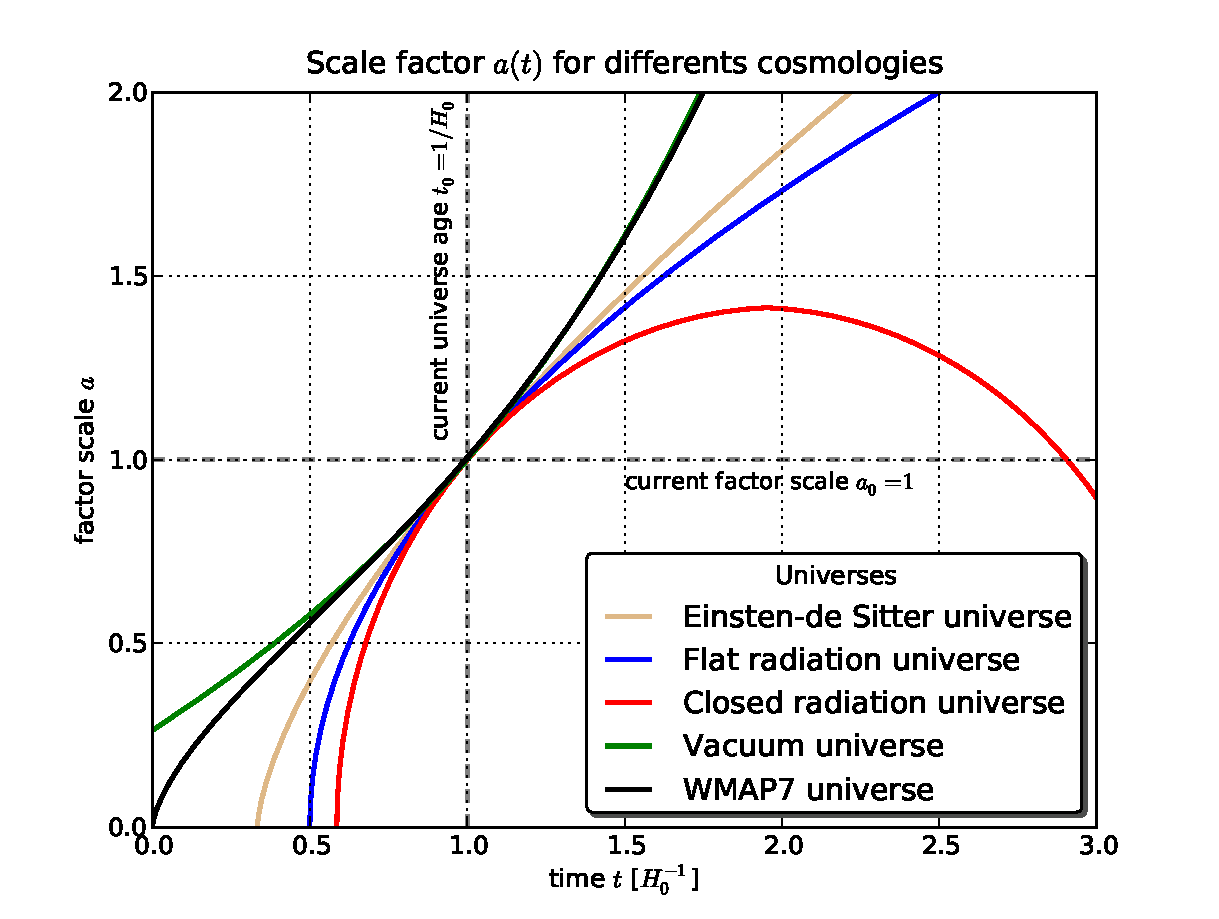
\includegraphics[width=0.9\textwidth]
	{./figures/2_theoretical_framework/Friedmann_Solution.pdf}

	\caption{\small{Diferentes soluciones de universo para las ecuaciones
	de Friedmann.}}
	
	\label{fig:Cosmologies}
\end{figure}
%.........................................................................
\

Es posible obtener una solución analítica de esta integral en términos de 
funciones elípticas, pero por simplicidad se opta por realizar una 
integración numérica. En la figura \ref{fig:Cosmologies} se muestra la 
solución para el universo WMAP7 y se compara con las demás cosmologías 
derivadas previamente.


Una característica interesante de la solución para un universo WMAP7 es
el cambio de concavidad (ver curva negra en la figura \ref{fig:Cosmologies})
que indica que se pasa de un régimen dominado por materia/radiación a uno 
dominado por la expansión acelerada asociada a la energía del vacío. 
Otro aspecto importante es la predicción de la edad el universo. Teniendo 
en cuenta la normalización definida anteriormente para el factor de escala 
$a(t_0) = a_0$, es directo ver que $t_0 = H_0^{-1} \approx 13.75 \times 10^9$ 
años. Otras cosmologías bajo la misma normalización predicen edades
diferentes, desde mayores como el caso del universo de vacío, hasta mucho 
menores e inclusive un tiempo final (big crunch) como el universo con 
geometría cerrada con radiación.


%*************************************************************************




%*************************************************************************
%Structure Formation
\section{Formación de Estructuras}
\label{sec:StructureFormation}


La sección pasada aborda el universo de manera completamente global, 
asumiendo válidas las condiciones de isotropía y homogeneidad. El 
universo real a pesar de tener ese comportamiento de manera asintótica en
escalas muy grandes, en escalas menores es muy diferente, siendo 
completamente anisotrópico y altamente no homogéneo. Un ejemplo claro de 
esto último es la vida, una de las más altas no linealidades del universo,
pasando luego por planetas, estrellas, galaxias, cúmulos galácticos, en 
orden de inhomogeneidad e anisotropía respectivamente.


La forma estándar de introducir estos efectos de estructura en el universo
es asumir válidas las soluciones de Friedmann a grandes escalas y considerar
las inhomogeneidades como perturbaciones del modelo. Pasando primero por el
régimen lineal para el cual las perturbaciones en el campo de densidad son 
mucho menores que el valor medio de fondo ($\delta \rho \ll \rho_b$)
subsección \ref{subsec:LinearEvolution}), hasta el régimen no lineal en que 
son comparables o mayores ($\delta \rho \sim \rho_b$) subsección 
\ref{subsec:NonLinearEvolution}).


	%---------------------------------------------------------------------
	%Linear Evolution
	\subsection{Evolución Lineal}
	\label{subsec:LinearEvolution}
	%---------------------------------------------------------------------


El marco de la evolución lineal puede ser abordado de dos formas. La primera
es considerar un término perturbativo en el tensor momentum-energía 
$ \delta T_{\mu \nu}$ y linealizar las ecuaciones de campo métrico 
\ref{eq:EinsteinEquations} y resolver finalmente para $\delta R_{\mu \nu}$


%.........................................................................
%Perturbative Einstein Equations
\eq{eq:PerturbativeEinsteinEquations}
{ \mathcal{L}( R_{\mu \nu}, \delta R_{\mu \nu} ) = 
\frac{8\pi G}{c^2}\pr{ T_{\mu \nu} + \delta T_{\mu \nu} } }
%.........................................................................


A pesar de que este método es rigurosamente más adecuado, tiene un 
incoveniente que lo hace considerablemente complicado de aplicar, los 
términos perturbativos no lo son necesariamente en todos los sistemas 
coordenados e incluso pueden llegar a ser del mismo orden o mayores que el 
término de fondo \cite{padmanabhan1995}.


El segundo método consiste en asumir perturbaciones con una dimensión 
comóvil menor al radio de Hubble ($r_\delta \ll r_H \sim cH_0^{-1}$) 
\footnote{Un radio de Hubble $r_H$ es una unidad de longitud que define 
el orden de magnitud del tamaño del universo observable.}, y así 
despreciar los efectos relativistas debido a la curvatura de la 
espacio-tiempo. Una vez hecho esto es posible usar un esquema Newtoniana 
para el desarrollo de las perturbaciones en el universo de fondo, este 
esquema asume el contenido de materia como un fluido y está soportado por 
tres ecuaciones básicas de la mecánica de fluidos. La primera es la 
ecuación de continuidad que representa la conservación de la masa del 
fluido


%.........................................................................
%Continuity equation
\eq{eq:ContinuityEquation}
{ \dtot{\rho}{t} = - \rho \nabla \cdot \bds u }
%.........................................................................


La segunda es la ecuación de Euler que caracteriza el campo de velocidades
del fluido y físicamente representa la conservación del momentum


%.........................................................................
%Euler Equation
\eq{eq:EulerEquation}
{ \dtot{\bds u}{t} = -\frac{ \nabla P}{\rho} - \nabla \phi }
%.........................................................................


Y finalmente la ecuación de Poisson que es la forma no relativista de las 
ecuaciones de campo de Einstein y especifica el contenido de materia como
fuentes de campo gravitacional.
	
	
%.........................................................................	
%Poisson Equation
\eq{eq:PoissonEquation}
{ \nabla^2 \varphi = 4\pi G \rho }
%.........................................................................	


Para completar el marco Newtoniano de perturbaciones es necesario incluir 
en el anterior sistema de ecuaciones (\ref{eq:ContinuityEquation}, 
\ref{eq:EulerEquation} y \ref{eq:PoissonEquation}) el efecto de la 
expansión del universo, para esto se realiza un cambio de coordenadas de
distancia propia $\bds x$ a distancia comóvil $\bds r$


%.........................................................................	
%Changing Coordinate
\[\bds x = a \bds r\]
%.........................................................................	


esto implica directamente que


%.........................................................................	
%Changing Coordinate
\[\bds u = \dtot{\bds x}{t} = 
\frac{\dot a}{a}\bds x + \bds v = \dot a \bds r + \bds v\]
%.........................................................................	


Esta forma de reescribir $\bds u$ permite separar la componente debida a la
expansión del universo ($\dot a/a \bds x$), o también denominada Ley de 
Hubble, de la componente debida al movimiento del fluido, denominado campo 
de velocidad peculiar y es definido como $\bds v = a \dot{ \bds r}$.

	
	%---------------------------------------------------------------------
	%Nonlinear Evolution
	\subsection{Evolución no Lineal}
	\label{subsec:NonLinearEvolution}
	%---------------------------------------------------------------------


%*************************************************************************




%*************************************************************************
%Quantification of cosmological environment
\section{Quantification of Cosmological Environment}
\label{sec:QuantificationOfCosmologicalEnvironment}


	%---------------------------------------------------------------------
	%The T-web method
	\subsection{The T-web Method}
	\label{subsec:TheT-webMethod}
	%---------------------------------------------------------------------


	%---------------------------------------------------------------------
	%The V-web method
	\subsection{The V-web Method}
	\label{subsec:TheV-webMethod}
	%---------------------------------------------------------------------


%*************************************************************************




%*************************************************************************
%Cosmological observations
\section{Observaciones Cosmológicas}
\label{sec:CosmologicalObservations}
	

%.........................................................................
%Cosmological Parameter of WMAP7
\begin{table}[htbp]
\begin{small}
\centering
\begin{tabular}{|c|c|c|c|} \hline
\cellc{\textbf{Parámetro}}		&
\cellc{\textbf{Notación}}		&  
\cellc{\textbf{Valor}}			& 
\cellc{\textbf{Unidades}}					\\ \hline


Edad del Universo  			&	$t_0$			&	$13.75 \pm 0.13$	&	Ga 				\\ \hline

Constante de Hubble			&	$H_0$			&	$71.0 \pm 2.5$		&   km/(Mpc s)		\\ \hline

Densidad de Bariones		&	$\Omega_b$		&	$0.0449\pm 0.0027$	&	--				\\ \hline

Densidad de & & & \\
Materia Oscura				&	$\Omega_c$		&	$0.222 \pm 0.026$	&	--				\\ \hline

Densidad de & & & \\
Energía Oscura				&	$\Omega_\Lambda$&	$0.734 \pm 0.029$	&	--				\\ \hline

Densidad de & & & \\
Radiación					&	$\Omega_r$		&$8.24 \times 10^{-5}$	&	--				\\ \hline

Amplitud de & & & \\
Fluctuaciones en $8h^{-1}$ Mpc&	$\sigma^2$		&	$0.801 \pm 0.030$	&	--				\\ \hline

Índice Espectral			&	$n_s$			&	$0.963 \pm 0.014$	&	--				\\ \hline
Profundidad Óptica & & & \\
de Reionización 			&	$\tau$			&	$0.088 \pm 0.015$	&	--				\\ \hline
				
Densidad Total & & & \\
del Universo	&	$\Omega_0$		&	$1.080\ \mbox{\scriptsize{$+0.093$}}/ 
										\mbox{\scriptsize{$-0.071$}} $&	--			\\ \hline
\end{tabular}
\caption{Parámetros cosmológicos WMAP7 \cite{WMAP7}.}
\label{tab:CosmologicalParameters}
\end{small}
\end{table}
%.........................................................................

%*************************************************************************